\section{Non-inverting Amplifier}

\subsection{Pengantar Non-Inverting Amplifier}
\begin{frame}{Pengantar Non-inverting Amplifier}
	\begin{itemize}
		\item Salah satu rangkaian op amp dasar
		\item Menggunakan negative feedback untuk menstabilkan overall voltage gain
		\item Negative feedback juga meningkatkan impedansi input dan menurunkan impedansi output
	\end{itemize}
\end{frame}

\subsection{Rangkaian Dasar}
\begin{frame}{Rangkaian Dasar}
	\begin{figure}
		\centering
		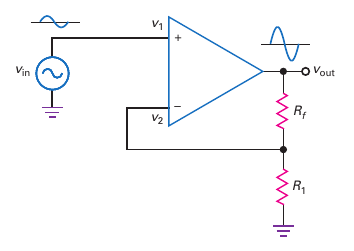
\includegraphics[width=0.5\linewidth]{gambar/fig-16.18}
		\caption{Non-inverting amplifier}
		\label{fig-16.18}
	\end{figure}
\end{frame}

\subsection{Virtual Short}
\begin{frame}{Virtual Short}
	\begin{multicols}{2}
		\begin{figure}
			\centering
			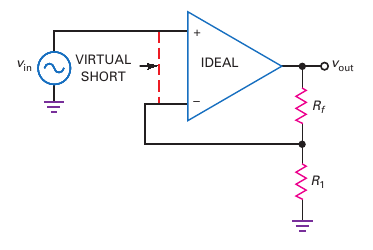
\includegraphics[width=\linewidth]{gambar/fig-16.19}
			\caption{Virtual short}
			\label{fig-16.19}
		\end{figure}
	\columnbreak
		\begin{itemize}
			\item Virtual short digunakan untuk menganalisis noninverting amplifier
			\item Virtual short berdasarkan 2 sifat dari op amp ideal
			\begin{enumerate}
				\item $ R_{in} = \infty \rightarrow i_1 = i_2 = 0$
				\item $ A_{VOL} = \infty \rightarrow v_1 - v_2 = 0$
			\end{enumerate}
		\end{itemize}
	\end{multicols}
\end{frame}

\subsection{Voltage Gain}
\begin{frame}{Voltage Gain}
	\begin{multicols}{2}
		\begin{figure}
			\centering
			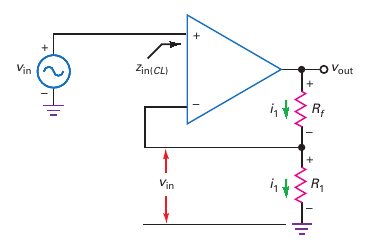
\includegraphics[width=\linewidth]{gambar/fig-16.20}
			\caption{Tegangan input ada di $ R_1 $ dan arus yang sama mengalir di $ R_1 $}
			\label{fig-16.20}
		\end{figure}
		\columnbreak
		\begin{itemize}
			\item Tegangan input: $ v_{in} = i_1 R_1 $
			\item Tegangan output: $ v_{out} = i_1 (R_f + R_1) $
			\item Penguatan tegangan closed-loop:
			\begin{align*}
				A_{v(CL)} = \frac{v_{out}}{v_{in}} = \frac{i_1 (R_f + R_1)}{i_1 R_1} = \frac{R_f + R_1}{R_1}
			\end{align*}
			maka
			\begin{equation}\label{pers.16.12}
				A_{v(CL)} = \frac{R_f}{R_1} + 1
			\end{equation}
		\end{itemize}
	\end{multicols}
\end{frame}

\subsection{Impedansi Input, Bandwidth, Bias \& Offset}
\begin{frame}{Impedansi Input, Bandwidth, Bias \& Offset}
	\begin{itemize}
		\item Karena impedansi input open-loop sudah sangat besar (2 M$ \Omega $ untuk 741C), maka impedansi input closed-loop lebih besar lagi.
		\item Efek negative feedback terhadap bandwidth sama seperti di inverting amplifier
		\[ f_{2(CL)} = \frac{f_{unity}}{A_{v(CL)}} \]
		\item Efek bias dan offset juga sama seperti di inverting amplifier
	\end{itemize}
\end{frame}

\subsection{Error Tegangan Output Mereduksi MPP}
\begin{frame}{Error Tegangan Output Mereduksi MPP}
	\begin{figure}
		\centering
		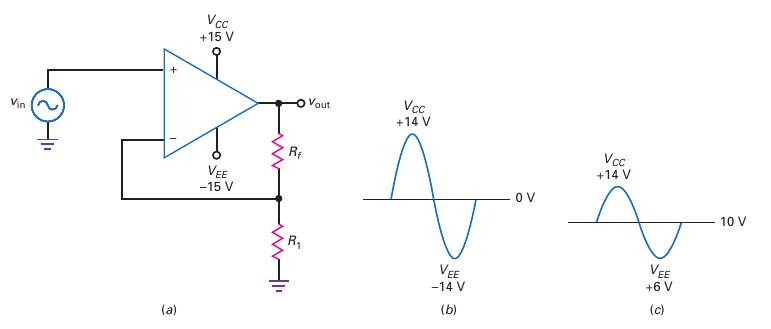
\includegraphics[width=0.9\linewidth]{gambar/fig-16.21}
		\caption{Error tegangan output dapat mereduksi MPP}
		\label{fig-16.21}
	\end{figure}
\end{frame}

\subsection{Contoh Soal 2.10}
\begin{frame}{Contoh Soal 2.10}
	\begin{multicols}{2}
		\begin{center}
			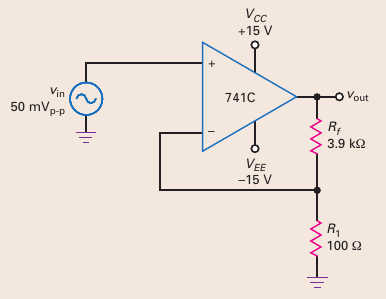
\includegraphics[width=\linewidth]{gambar/fig-16.22a}
		\end{center}
		\columnbreak
		\begin{itemize}
			\item Pertanyaan:
			\begin{itemize}
				\item Berapa penguatan tegangan closed-loop dan bandwidth?
				\item Berapa tegangan output di 250 kHz?
			\end{itemize}
		\end{itemize}
	\end{multicols}
\end{frame}

\begin{frame}{Contoh Soal 2.10}
	\begin{multicols}{2}
		\begin{center}
			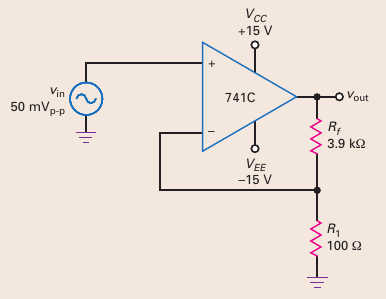
\includegraphics[width=\linewidth]{gambar/fig-16.22a}
		\end{center}
		\columnbreak
		\begin{itemize}
			\item Jawaban:
			\begin{itemize}
				\item Penguatan tegangan closed-loop:
				\begin{align*}
					A_{v(CL)} &= \frac{R_f}{R_1} + 1 = \frac{3.9 \text{ k}\Omega}{100 \text{ k}\Omega} + 1 \\
					&= 40
				\end{align*}
				\item Bandwidth:
				\begin{align*}
					f_{2(CL)}
				\end{align*}
			\end{itemize}
		\end{itemize}
	\end{multicols}
\end{frame}